\documentclass{article}
\usepackage{graphicx}
\graphicspath{ {./img/} }

\title{Design Plan}
\author{SPC James Viner, SPC Jeremy Carter, CW2 Richard Soto}
\date{Thursday, April 20, 2023}

\begin{document}
  \maketitle
  \section*{Project Summary}
  A pair of programs, a dispatcher and a listener, will act as a communication relay.
  The program dispatcher passively accepts text from standard input, exiting normally on EOF.
  The program listener will print out any text that was sent to a running instance of dispatcher. When
  dispatcher exits, so too does listener.

  \begin{figure}[h]
  \caption{Overall Workflow of Program}
  \centering
  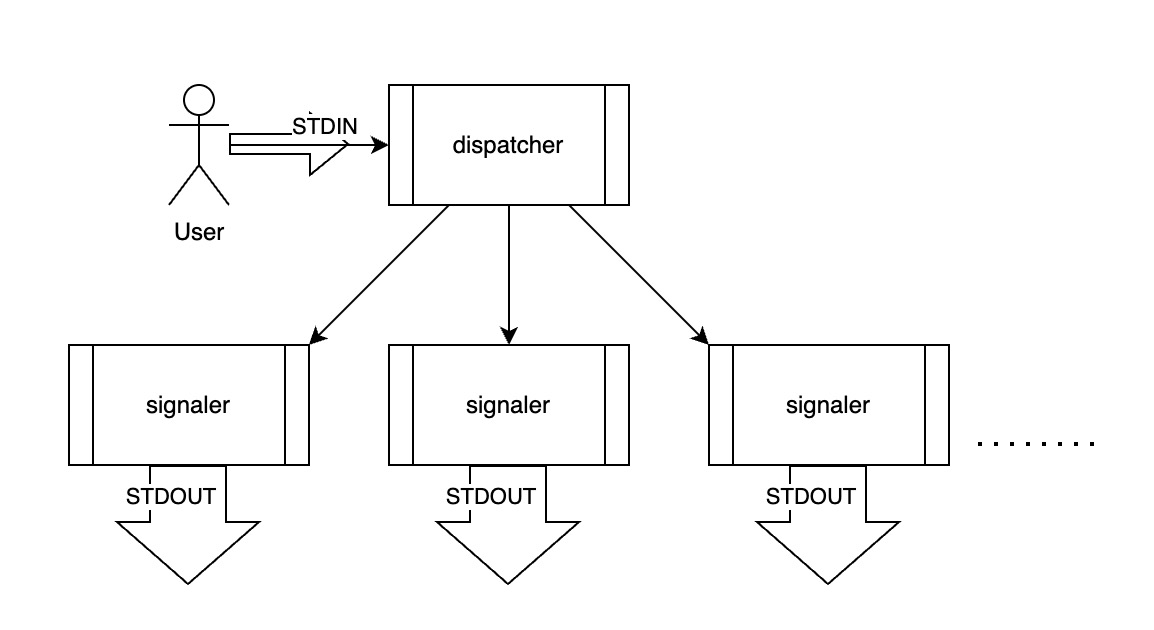
\includegraphics[width=0.5\textwidth]{app_img}
  \end{figure}


  \section*{Features Targeted}
  \subsection*{Man Page}
  Make a sample man page for the program that explains how it works and any errors it may return.
  \subsection*{LaTeX Design Plan/Write Up}
  Have the Project write up and design plan in LaTeX code.
  \subsection*{Multiple instances of listener to connect}
  Allow for multiple instances of listener to connect to a single instance of
  dispatcher. All instances of listener should print the text read by dispatcher.
  \subsection*{-l flag}
  Add a -l <n> flag to dispatcher
  that specifies the maximum number of listener instances. Any additional
  listener instances that attempt to start should exit with an appropriate error
  message.
  \subsection*{-b flag}
  Add a -b flag to dispatcher which allows it to read from stdin without buffering
  by line (See termios(3) or ncurses(3)).

  \section*{Architecture}
  \subsection*{Data}
Two structs will be used; one for the flags on the command line and one for details related to the message.\\
struct msg{\\
\qquad \indent int msg\_code\\
\qquad \indent char *msg\\
\qquad \indent size\_t msg\_sz\\
}\\
struct app{\\
\qquad \indent int num\_list\\
\qquad \indent bool flag\_no\_buff\\
}\\
  \subsection*{Significant Functions}
  char * get\_input(void)\\
  \qquad \indent This function will get input from the user.\\
  void brdcst\_msg(void)\\
  \qquad \indent This function will send the message out to all connected clients.\\
  void create\_socket(void)\\
  \qquad \indent This function will set up the Unix socket.\\
  void signal\_handler()\\
  \qquad \indent This function will handle any signals that are sent to the program.\\
  int tear\_down(void)\\
  \qquad \indent This function will close the socket and free any memory that was allocated as well as closing
  the clients.\\
  int connect\_svr(void)\\
  \qquad \indent This function will connect to the server.\\
  void print\_msg(char *msg)\\
  \qquad \indent This function will print the message to the screen.\\

  \section*{Plan}
  The plan for this project is to start with standing up the server and ensuring a single client
  can connect and receive messages. Once this is successful, we will focus on allowing multiple
  connections to the server. Once this is successful, we will focus on adding the flags and
    ensuring that the server can handle multiple clients. Finally, we will ensure that the server
    can successfully broadcast a signal to inform the clients to shutdown.
  \section*{User Interface}
Uses the CLI. The user will initiate the program with no flags/one flag/multiple flags. The user
will then input text via the terminal. The program will not end until the proper signal is sent
by the user to the program.
\\
\\
\end{document}

